\documentclass[10pt, aspectratio=169]{beamer}
\usepackage{beamerthemeMathFest}
\usepackage{tcolorbox}
\usepackage{physics}
\usepackage{booktabs}
\usetikzlibrary{arrows.meta, calc, positioning}
\definecolor{TimeSeriesRed}{HTML}{D55E00}
\definecolor{TimeSeriesBlue}{HTML}{0072B2}

\title[Reservoir Computers and Causal States]{The Quality of a Reservoir Computer is Determined by its Relationship to Causal States}
\subtitle{MAA Socal-NV Section Meeting at CSULA, Los Angeles, CA}

\author{Christopher Wang}
\institute{Scripps College}
\date{October 24, 2026}

\graphicspath{figs/}

\begin{document}

\maketitle

\section{Background}

\begin{frame}{Motivation}
\begin{center}
	\begin{tcolorbox}[colback=red!10!white, colframe=red!50!black, left=1mm, right=1mm, arc=2mm]
		\centering
		\resizebox{\linewidth}{!}{\textcolor{red!50!black}{\textbf{How do complex systems, such as artificial neural networks, predict effectively?}}}
	\end{tcolorbox}
	\vspace{2em}
\end{center}
\pause

\textbf{Scope:} we investigate prediction in time series.
\end{frame}

\begin{frame}{Modeling Time Series: Edge-Emitting Hidden Markov Models}
	\begin{columns}[c,onlytextwidth]
		\begin{column}{0.43\textwidth}
			\centering
			\resizebox{0.95\linewidth}{!}{%
				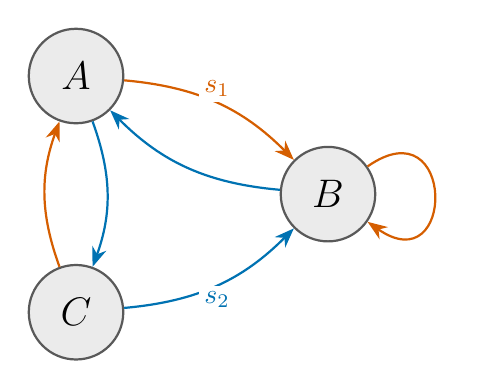
\begin{tikzpicture}[
					state/.style={circle, draw=black!65, fill=black!8,
						thick, minimum size=12mm, inner sep=2pt, font=\Large},
					transition/.style={-{Stealth[length=2.5mm]}, thick}
				]
					\node[state] (a) at (0,1.5) {$A$};
					\node[state] (b) at (3.2,0) {$B$};
					\node[state] (c) at (0,-1.5) {$C$};
					\path[transition,color=TimeSeriesRed]
						(a) edge[bend left=20]
							node[midway,above,fill=white,inner sep=2pt,text=TimeSeriesRed] {$s_1$} (b)
						(b) edge[out=35,in=-35,looseness=5] (b)
						(c) edge[bend left=20] (a);
					\path[transition,color=TimeSeriesBlue]
						(a) edge[bend left=20] (c)
						(b) edge[bend left=20] (a)
						(c) edge[bend right=20]
							node[midway,below,fill=white,inner sep=2pt,text=TimeSeriesBlue] {$s_2$} (b);
				\end{tikzpicture}%
			}
		\end{column}
		\begin{column}{0.53\textwidth}
			\begin{itemize}\addtolength{\itemsep}{1em}
				\item Observations: $\{\textcolor{TimeSeriesRed}{s_1},\textcolor{TimeSeriesBlue}{s_2}\}$
				\item Hidden states: $G=\{A,B,C\}$
				\item Observation emitted while transitioning between states
				\pause
				\item \textbf{What artificial neural network can be used to predict observables?}
			\end{itemize}
		\end{column}
	\end{columns}
\end{frame}

\begin{frame}{Reservoir Computers: a Special Recurrent Neural Network}
\begin{columns}
	\begin{column}{0.45\textwidth}
		\begin{itemize}
			\item Recurrent Neural Networks (RNNs):
			\begin{itemize}
				\item Best for time series prediction
				\item Traditional architectures have mathematical problems
			\end{itemize}
			\pause
			\item Reservoir Computers \cite{jaeger2001}
			\begin{itemize}
				\item Fixed hidden layer connectivity
				\item Linear output layer $\hat{y} = W^\text{out}\vb{x}$
			\end{itemize}
			\pause
			\item Recurrence relation:
			\begin{equation}
				\vb{x}_{t+1} = f(W \vb{x_t} + W^\text{in} \vb{u}_{t+1}).
			\end{equation}
			\begin{itemize}
				\item $\vb{x}$: Reservoir state
				\item $\vb{u}$: Input
				\item $W, W^\text{in}$: Reservoir matrices
				\item $f$: Reservoir activation function
			\end{itemize}
		\end{itemize}
	\end{column}
	\hfill
	\begin{column}{0.45\textwidth}
		\begin{figure}
			\centering
			\setbeamertemplate{caption}{\centering\footnotesize\insertcaption\par}
			\resizebox{\linewidth}{!}{%
				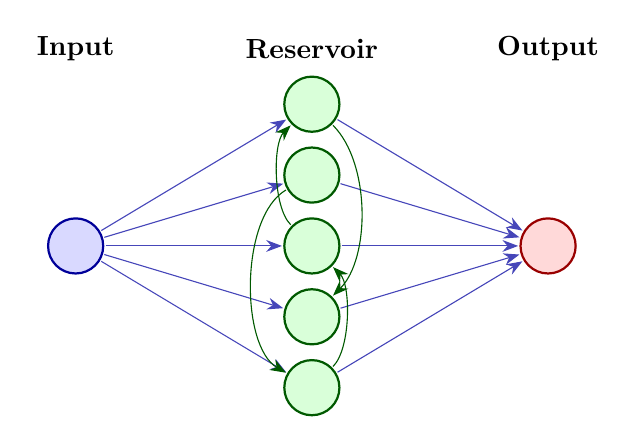
\begin{tikzpicture}[
					neuron/.style={circle, draw, thick, minimum size=7mm, inner sep=0pt},
					connection/.style={-{Stealth[length=2mm]}, thin, shorten <=3.8mm, shorten >=3.8mm},
					feedforward/.style={connection, draw=blue!45!gray},
					recurrent/.style={connection, draw=green!35!black}
				]
					\coordinate (input) at (0,0);
					\coordinate (r1) at (3,1.8);
					\coordinate (r2) at (3,0.9);
					\coordinate (r3) at (3,0);
					\coordinate (r4) at (3,-0.9);
					\coordinate (r5) at (3,-1.8);
					\coordinate (output) at (6,0);

					\foreach \i in {1,...,5} {
						\draw[feedforward] (input) -- (r\i);
						\draw[feedforward] (r\i) -- (output);
					}
					\draw[recurrent] (r3) to[bend left=45] (r1);
					\draw[recurrent] (r5) to[bend right=45] (r3);
					\draw[recurrent] (r1) to[bend left=45] (r4);
					\draw[recurrent] (r2) to[bend right=60] (r5);

					\node[neuron, draw=blue!60!black, fill=blue!15] at (input) {};
					\foreach \i in {1,...,5} {
						\node[neuron, draw=green!35!black, fill=green!15] at (r\i) {};
					}
					\node[neuron, draw=red!60!black, fill=red!15] at (output) {};
					\node[font=\bfseries] at (0,2.5) {Input};
					\node[font=\bfseries] at (3,2.5) {Reservoir};
					\node[font=\bfseries] at (6,2.5) {Output};
				\end{tikzpicture}%
			}
			\caption{A simple illustration of a reservoir computer.}
		\end{figure}
		\vspace{-1em}
		\pause
		\begin{itemize}
			\item \textbf{How does one predict?}
		\end{itemize}
	\end{column}
\end{columns}
\end{frame}


\begin{frame}{Computational Mechanics and Causal States \cite{shalizi2001}}
	\begin{columns}[T,onlytextwidth]
		\begin{column}{0.39\textwidth}
			\centering
			\textbf{Histories $\overleftarrow{\boldsymbol{\mathcal{S}}}$}\par
			\medskip
			\resizebox{0.90\linewidth}{!}{%
				\begin{tikzpicture}
					\def\historyblob{(0.2,2.4)
						.. controls (0.05,3.4) and (0.9,4.3) .. (1.9,4.1)
						.. controls (2.7,3.9) and (3.2,4.6) .. (4.2,3.9)
						.. controls (5.1,3.4) and (4.5,2.8) .. (4.8,2.1)
						.. controls (5.1,1.1) and (4.0,0.45) .. (3.1,0.7)
						.. controls (2.2,0.95) and (1.6,0.2) .. (0.8,0.9)
						.. controls (0.05,1.4) and (0.45,1.8) .. (0.2,2.4) -- cycle}
					\begin{scope}
						\clip \historyblob;
						\fill[MathBlue!18] (-1,0) rectangle (6,5);
						\fill[MathGreen!30] (-1,2.5)
							.. controls (0.7,2.8) and (1.6,2.2) .. (2.5,2.5)
							.. controls (2.2,3.2) and (2.9,3.9) .. (2.8,5)
							-- (-1,5) -- cycle;
						\fill[orange!22] (-1,2.5)
							.. controls (0.7,2.8) and (1.6,2.2) .. (2.5,2.5)
							.. controls (2.8,1.8) and (2.35,1.0) .. (2.7,0)
							-- (-1,0) -- cycle;
						\draw[MathGreenDark, thick] (2.8,5)
							.. controls (2.9,3.9) and (2.2,3.2) .. (2.5,2.5)
							.. controls (2.8,1.8) and (2.35,1.0) .. (2.7,0);
						\draw[MathGreenDark, thick] (-1,2.5)
							.. controls (0.7,2.8) and (1.6,2.2) .. (2.5,2.5);
					\end{scope}
					\draw[MathGreenDark, very thick] \historyblob;
					\node[font=\Large] at (1.35,3.35) {$\sigma_1$};
					\node[font=\Large] at (1.35,1.55) {$\sigma_2$};
					\node[font=\Large] at (3.65,2.5) {$\sigma_3$};
				\end{tikzpicture}%
			}
		\end{column}
		\begin{column}{0.58\textwidth}
			\footnotesize
			For $\overleftarrow{s},\overleftarrow{s}'\in\overleftarrow{\boldsymbol{\mathcal{S}}}$, define
			\begin{align*}
				\overleftarrow{s}\sim_\epsilon\overleftarrow{s}'
				\quad &\Longleftrightarrow \\[0.3em]
				P\!\left(\overrightarrow{S}^{L}=\overrightarrow{s}^{L}
				\mid\overleftarrow{S}=\overleftarrow{s}\right)
				&=P\!\left(\overrightarrow{S}^{L}=\overrightarrow{s}^{L}
				\mid\overleftarrow{S}=\overleftarrow{s}'\right)
			\end{align*}
			% \vspace{-0.8em}
			for every $L\geq1$ and every future $\overrightarrow{s}^{L}$. Histories with the same future distribution form one causal state.

			\medskip
			{\footnotesize
			\textbf{Notation}\par\smallskip
			\begin{tabular}{@{}l@{\quad}l@{}}
				$\overleftarrow{\boldsymbol{\mathcal{S}}}$ & Set of all histories\\[0.25em]
				$\overleftarrow{S}, \overleftarrow{s}$ & Random history, a specific history\\[0.25em]
				$\overrightarrow{S}^{L}, \overrightarrow{s}^{L}$ & Random length-$L$ future, a specific length-$L$ future\\[0.25em]
				$L,\ \sigma_i$ & Future length, a causal state
			\end{tabular}}
		\end{column}
	\end{columns}
	\smallskip
	\begin{tcolorbox}[colback=MathGreen!15, colframe=MathGreenDark,
		left=1mm, right=1mm, top=1mm, bottom=1mm, arc=2mm]
		\centering\bfseries
		Causal states are the minimal sufficient statistics of prediction.
	\end{tcolorbox}
\end{frame}

\begin{frame}{The $\varepsilon$-machine}
	\begin{columns}[c,onlytextwidth]
		\begin{column}{0.43\textwidth}
			\centering
			\resizebox{0.96\linewidth}{!}{%
				\begin{tikzpicture}[
					state/.style={circle, draw=MathGreenDark, thick,
						minimum size=12mm, inner sep=2pt, font=\Large},
					transition/.style={-{Stealth[length=2.5mm]},
						color=MathBlue!65!gray, thick}
				]
					\node[state, fill=MathGreen!30] (s1) at (0,1.5) {$\sigma_1$};
					\node[state, fill=orange!22] (s2) at (0,-1.5) {$\sigma_2$};
					\node[state, fill=MathBlue!18] (s3) at (3.2,0) {$\sigma_3$};
					\path[transition]
						(s1) edge[out=120,in=190,looseness=5] (s1)
						(s1) edge[bend left=20]
							node[midway,above,fill=white,inner sep=2pt,text=black] {$u$} (s3)
						(s3) edge[bend left=20] (s1)
						(s3) edge[out=35,in=-35,looseness=5] (s3)
						(s2) edge[bend left=20] (s1)
						(s3) edge[bend left=20] (s2);
				\end{tikzpicture}%
			}
			\medskip
			$u$: emitted symbol
		\end{column}
		\pause
		\begin{column}{0.54\textwidth}
			\resizebox{\linewidth}{!}{%
				If $\boldsymbol{\mathcal{S}}=\{\sigma_1,\sigma_2,\sigma_3\}$
				and $\mathbf{T}\triangleq\text{transitions}$,%
			}
			\[
				\varepsilon\text{-machine}:\;
				\{\boldsymbol{\mathcal{S}},\mathbf{T}\}
			\]

			\bigskip
			The $\varepsilon$-machine is \emph{deterministic}.
		\end{column}
	\end{columns}
\end{frame}

\begin{frame}{Process Generation: Hidden Markov Models (HMMs)}
	\begin{columns}[c,onlytextwidth]
		\begin{column}{0.46\textwidth}
			\centering
			\textbf{Simple nonunifilar source}\par
			\medskip
			% Source: https://redwood.berkeley.edu/wp-content/uploads/2018/01/marzen2015informational.pdf, Fig. 2(b).
			\resizebox{0.95\linewidth}{!}{%
				\begin{tikzpicture}[
					state/.style={circle, draw=MathGreenDark, thick,
						minimum size=12mm, inner sep=2pt, font=\Large},
					transition/.style={-{Stealth[length=2.5mm]},
						color=MathBlue!65!gray, thick},
					label/.style={font=\small, text=black, fill=white, inner sep=2pt}
				]
					\node[state, fill=MathGreen!30] (a) at (0,0) {$A$};
					\node[state, fill=MathBlue!18] (b) at (3.2,0) {$B$};
					\path[transition]
						(a) edge[out=125,in=235,looseness=5]
							node[label,left] {$\tfrac12:0$} (a)
						(a) edge[bend left=25]
							node[label,midway,above] {$\tfrac12:0$} (b)
						(b) edge[bend left=25]
							node[label,midway,below] {$\tfrac12:1$} (a)
						(b) edge[out=55,in=-55,looseness=5]
							node[label,right] {$\tfrac12:0$} (b);
				\end{tikzpicture}%
			}
			\smallskip
			{\footnotesize Edge labels: probability : symbol}\par
			\bigskip
			{\large Emission stream: $\cdots010000101\cdots$}
		\end{column}
		\begin{column}{0.50\textwidth}
			\begin{itemize}\addtolength{\itemsep}{1.5em}
				\item Process generator not deterministic!
				\item $\varepsilon$-machine: belief states $\mu(g)$, $g \in G = \{A,B\}.$
			\end{itemize}
		\end{column}
	\end{columns}
\end{frame}

\section{Contributions}

\begin{frame}{Making the Optimal Prediction}
	\begin{itemize}\addtolength{\itemsep}{10pt}
		\item \textbf{Assumptions:}
		\begin{itemize}
			\item $u$ is scalar
			\item Aim to minimize future $u(t+\tau)$ via mean-square error
		\end{itemize}
		\pause
		\item Best estimate: $\mathbb{E}[u(t+\tau) \mid \sigma(t)]$
		\pause
		\item Conceptually...
		\begin{itemize}
			\item Advance $\sigma(t) \longrightarrow \sigma(t+\tau)$
			\item Inner product with emission probabilities $p(u \mid g)$
			\item Weighted sum/integral over emissions $u$
		\end{itemize}
		\pause
		\item Here, $\sigma(t)$ is a measure on $G$ at time $t$
	\end{itemize}
\end{frame}

\begin{frame}{The Optimal Prediction: A Mathematical Form}
	\begin{align}
		\mathbb{E}[u(t+\tau) \mid \sigma(t)] &= \int \left< (\mathcal{T}^\tau \mu)(g), p(u \mid g) \right>_G u\, \dd u \\[0.8em]
		\left< (\mathcal{T}^\tau \mu)(g), p(u \mid g) \right>_G &= \int_G p(u \mid g) \, \dd(\mathcal{T}^\tau \mu)(g)
	\end{align}
	\begin{itemize}
		\item $\mathcal{T}^\tau$: transition operator on $\mu$ (generalization of $\mathbf{T}$)
		\item $u$: input/emission
		\item $g$: element of the generative model $G$
		\item $\left< \cdot, \cdot \right>_G$: inner product over $G$
	\end{itemize}
\end{frame}

\begin{frame}{Lorenz System: An Example}
	\begin{columns}
		\begin{column}{0.45\textwidth}
		\begin{itemize}\addtolength{\itemsep}{8pt}
			\item Approximation of atmospheric convection model
			\item \emph{Deterministic} system of coupled ODEs in 3D
			\item Input: $x$ coordinate of Lorenz system
			\item Causal states: present-time coordinates $\vb{x}=(x,y,z)$
			\item Optimal prediction: $\mathbb{E}[u(t+\tau) \mid \sigma(t)] = x(t+\tau)$
		\end{itemize}
		\end{column}
		\hfill
		\begin{column}{0.45\textwidth}
			\centering
			\resizebox{\linewidth}{!}{%
				\begin{tikzpicture}[x=0.14cm,y=0.10cm]
					\draw[MathBlue!80!black, line width=0.25pt, line join=round]
						plot file {figs/lorenz-attractor.dat};
				\end{tikzpicture}%
			}
		\end{column}
	\end{columns}
\end{frame}

\begin{frame}{Lorenz System: An Example}
	\begin{itemize}\addtolength{\itemsep}{8pt}
		\item The measure $\mu(g)$ is the Dirac measure $\delta_{\vb{x}}$
		\item Operator $\mathcal{T^\tau}$ is the Lorenz flow
		\item Emission probability is $p(x \mid \vb{x}') = \delta(x-x')$
	\end{itemize}
	\bigskip
	\begin{align}
        \mathbb{E}[u(t+\tau) \mid \sigma(t)] &= \int_\mathbb{R} \left< (\mathcal{T}^\tau \mu)(\vb{x}'), p(x \mid \vb{x}') \right>_{\mathbb{R}^3} x \, \dd x \\
        &= \int \left( \int \delta(x-x') \dd \delta_{\vb{x}(t+\tau)} \right) x \, \dd x \\
        &= \int \delta(x-x(t+\tau))\, x \, \dd x \\
        &= x(t+\tau).
\end{align}
\end{frame}

\begin{frame}{An Optimally Predicting Reservoir Must Contain Causal States}
	\begin{equation}
		\mathbb{E}[u(t+\tau) \mid \sigma(t)] = W^\text{out}(\tau)\vb{x}(t)
	\end{equation}
	\vspace{0.5cm}
	\begin{center}
		This must hold for all $\tau\quad\implies\quad \vb{x}$ must contain representation of causal states!  
	\end{center}
\end{frame}

\section{Acknowledgements}

\begin{frame}{Acknowledgements}
	\begin{itemize}\addtolength{\itemsep}{10pt}
		\item PI: Sarah Marzen
		\item Co-authors: Ambika Tiwari, Alicia Luo, Soren Cabinte, Sagun Bhandari, Marcelo Amaral, Sarah Marzen
	\end{itemize}
\end{frame}

\begin{frame}{Bibliography}
	\setbeamertemplate{bibliography item}{\insertbiblabel}
	\setbeamercolor{bibliography entry author}{fg=black}
	\setbeamercolor{bibliography entry location}{fg=black}
	\setbeamercolor{bibliography entry note}{fg=black}
	\begin{thebibliography}{2}
		\bibitem{jaeger2001}
		Herbert Jaeger.
		\newblock The ``echo state'' approach to analysing and training recurrent neural networks.
		\newblock GMD Report 148, German National Research Center for Information Technology, 2001.
		\newblock \href{https://doi.org/10.24406/publica-fhg-291111}{doi:10.24406/publica-fhg-291111}.

		\vspace{1em}
		\bibitem{shalizi2001}
		Cosma Rohilla Shalizi and James P. Crutchfield.
		\newblock Computational Mechanics: Pattern and Prediction, Structure and Simplicity.
		\newblock \emph{Journal of Statistical Physics}, 104:817--879, 2001.
		\newblock \href{https://arxiv.org/abs/cond-mat/9907176}{arXiv:cond-mat/9907176}.
	\end{thebibliography}
\end{frame}

{\BackgroundShaded
\begin{frame}
\begin{center}
	\Large{\textcolor{white}{Thank you!}}
\end{center}
\vspace{1cm}
{\footnotesize \textcolor{white}{Sponsored by ARO Grant W9111NF-25-1-0260.}}
\end{frame}}

\end{document}
